% This is LLNCS.DEM the demonstration file of
% the LaTeX macro package from Springer-Verlag
% for Lecture Notes in Computer Science,
% version 2.4 for LaTeX2e as of 16. April 2010
%
\documentclass{llncs}
%
\usepackage{graphicx}
\usepackage{amsmath}

%\usepackage{makeidx}  % allows for indexgeneration
%
\begin{document}
%
\frontmatter          % for the preliminaries
%
\pagestyle{headings}  % switches on printing of running heads
\addtocmark{Non-Parametric Transformation Networks} % additional mark in the TOC
%
\mainmatter              % start of the contributions
%
\title{Non-Parametric Transformation Networks}
%
\titlerunning{Non-Parametric Transformation Networks}  % abbreviated title (for running head)
%  
%
\author{Daniel Biskup and Catherine Capellen}
%
\authorrunning{Daniel Biskup and Catherine Capellen} % abbreviated author list (for running head)
%
%%%% list of authors for the TOC (use if author list has to be modified)
\tocauthor{Daniel Biskup and Catherine Capellen}
%
\institute{University of Bonn}

\maketitle              % typeset the title of the contribution

\begin{abstract}
The abstract 
\end{abstract}
%

\section{Introduction}
GENERAL TOPIC: Object recognition, CNNs, POOLING, PTN/NPTN, Paper results (SHORT) 
TASK
ROTNET TASK

\section{Related Work}
in lab report ? ( DO WE NEED THIS SECTION?) Maybe mention Spatial-
Transformer networks?

\section{Networks Architectures ( aka Methods)}
The kinds of networks this report is concerned with are Convolutional Neueral Networks (CNNs), Non-Parametric Transformation Networks (NPTNs), a custom network architecture we call RotNets.

\subsection{Convolutional Neueral Networks}
NPTNs can be seen as a generalization of CNNs. For that reason we will briefly discuss CNNs.
\subsubsection{Convolution}
As the name suggests, NPTSn make heavy use of the Convolution Operation. Convolutions calculate the weighted sum over a sub region of an input image in order to calculate the pixel-values of the output. The weights used for calculation the weighted sum are given by a matrix called filter or ”Kernel. Naturally different Kernels produce different results. In Computer Vision they are used to detect different kinds patterns. Thus one kernel might respond to vertical edges, another  one to horizontal edges and yet another one to yet another pattern. While kernels traditionally got designed by experts in Computer Vision, whithin CNNs they are expected to be learned by the network.
%TODO Add Conv graphic
\subsubsection{Spatial Max Pooling}
Another important operation used in CNNs is Max Pooling.
Each neuron in the max pooling layer connevts to a region of the previous
layer and only take the maximum output. By doing this they make the network
invariant to small translations

\subsection{Non-Parametric Transformation Networks}
\begin{itemize}
  \item	mathmotivation
  \item Architecture
  \item How they are a generalization of CNNs
\end{itemize}

\subsection{RotNets}
Loremipsum

\section{Implementation in with PyTorch}
Because the authors of the paper in NPTNs state, that they used PyTorch for their experiments, and because PyTorch is widely accepted and adopted within the scientific community, we decided to base our experiments on PyTorch as well.
To be able to reproduce the experiments performed in the paper, we had to implement the NPTN layer. To see if our approach, the RotNet, would perform well we had to implement it as well.
\subsection{The NPTN Layer}
%TODO Add NPTN graphics!
Lets say we have M inputs and want N outputs while using a set of G different filters for each path from input to output.
Just as for CNNS, all filters we use during convolution are also parameters that are expected to be learned by the network.
For this reason we can perform the convolutions by using an instance of the nn.Conv2d layer which will automatically initialize the filters and also register them as learn able parameters.

with M inputs and M*N*G outputs. The important implementation detail here is, that
we need to set the groups option to M, which causes Conv2d to use a filter bank
of N*G filters per input.
Right now we have N packs of G layers of one input stacked on each other
but we want G layers of input 1 are followed by G layers of input 2 and so on.
This can be archived by a simple permutation.
Next we use MaxPool3d with stride 1 and kernel size (G,1,1), that is NOT
spatial max pooling, but instead max pooling across the layers! Basically calcu-
lating the pixel wise maximum of G consecutive layers.
This is followed by the Average Pooling across layers, which is common to
CNNs.
As a side note: All those operations are tracked by pyTorchs AutoGrad which
allows calculating the gradiands for BackPropagation.
This concludes the implementation of the NPTN layer.

But to run actual experiments, you need to stack multiple network layers on
top of each other. And this is where the paper gave us a hard time, because it
didnt specify the size of each layer precisely enough. So we had to try to guess
which filter sizes they used.

\subsection{The RotNet Layer}
DETERMINATION OF NETWORK DIMENSION (48,16): EQUAL AMOUNT
OF PARAMETERS
ROTNET: GRIDSAMPLER, DIFFERENTIABLE
(DIMENSION DING)
NPTN IMPLEMENTATION

\subsubsection{The convolution}
Within the implementation of the NPTN layer we were able to use an instantiation of the nn.Conv2d layer, because we had to learn each kernel we used individually, i.e every kernel used for convolution was also a parameter of the network.\\
For the RotNet layer on the other hand, we need to use the nn.functional.conv2d function which expacts as argument the kernels we want to use, while inside the definition of the NPTN layers class we only "mark" the unrotated kernels as parameters by calling "" on them.

\subsubsection{GRIDSAMPLER, DIFFERENTIABLE}
\subsubsection{DETERMINATION OF NETWORK DIMENSION (48,16): EQUAL AMOUNT OF PARAMETERS}

4 EXPERIMENTS
- DESIGN (WHAT WAS IN PAPER AND WHAT WASN'T)

\section{Experiments and Results}	
In the following we will present three experiments from the paper that we tried to reproduce and tried to mimic as closely as possible. 
All the experiments use a two-layered or three-layered structure which include either a NPTN layer, a Convolutional layer or a RotNet layer in each layer. The structure for the two-layered network is shown in Figure \ref{pic:net_structure}. The last softmax layer is not described in the paper, but was added by us [WHY softmax, because it's standard]. 

\begin{figure}
	\begin{center}
	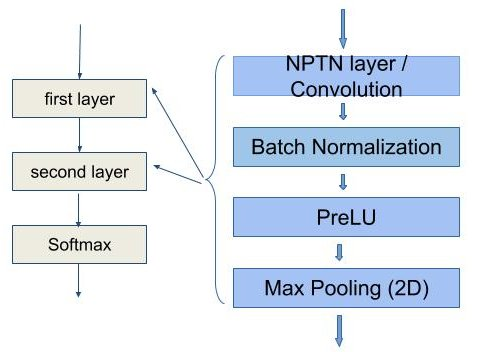
\includegraphics[scale=0.35]{result_images/network_structure.jpg}
	\caption{Structure of a two layered network.}
	\label{pic:network_structure}
	\end{center}
\end{figure}

\subsection{Experiments on CIFAR10}
The first experiment used the CIFAR10 dataset [CITE]. 
The paper describes in detail the setup of the experiments regarding learning rate, data preprocessing and network dimensions. However other important information as filter size and loss function is missing. 
For the filtersize we used 5, since in the other experiments, the paper mentions  filtersizes of 3,5 or 7 and 5 often shows the best performance for the NPTNs. 
In Figure \ref{pic:first_experiment} we show the results from the paper next to our experimental results. For the loss function we chose Negative Log Likelihood Loss (NLLL) [WHY]. 
However we did not get any comparable loss values as in the paper. Comparing the loss values of the networks to each other, in the paper, all NPTNs perform better than the CNN. In our results, only one of the NPTNs performs better.


\begin{figure}
	\begin{center}
	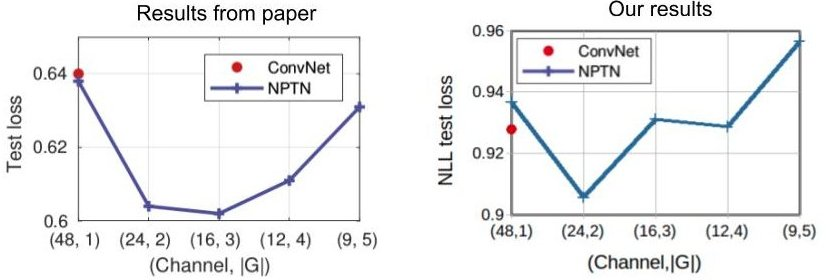
\includegraphics[scale=0.35]{result_images/experiment1.jpg}
	\caption{The first experiment}
	\label{pic:first_experiment}
	\end{center}
\end{figure}

TRAIN vs TEST ERROR?

CONCLUSION: PAPER IS NOT REPRODUCABLE
NPTNs FROM THIS EXPERIMENTS NOT BETTER 
(
ROTNET BAD

\section{Conclusion}
TRAIN vs TEST ERROR?
CONCLUSION: PAPER IS NOT REPRODUCABLE NPTNs FROM THIS
EXPERIMENTS NOT BETTER ( ROTNET BAD
\section{Discussion and further work}
WHY WE THINK NPTNS ARE LESS POWERFULL WHY ROTNETS ARE
WORSE THAN NPTNs WHY IT IS MAYBE NOT A GOOD IDEA TO RO-
TATE EARLY FILTERs
%
% ---- Bibliography ----
%
\begin{thebibliography}{}
%
\bibitem[1980]{2clar:eke}
Clarke, F., Ekeland, I.:
Nonlinear oscillations and
boundary-value problems for Hamiltonian systems.
Arch. Rat. Mech. Anal. 78, 315--333 (1982)

\end{thebibliography}
%\clearpage
%\addtocmark[2]{Author Index} % additional numbered TOC entry
%\renewcommand{\indexname}{Author Index}
%\printindex
%\clearpage
%\addtocmark[2]{Subject Index} % additional numbered TOC entry
%\markboth{Subject Index}{Subject Index}
%\renewcommand{\indexname}{Subject Index}
%%                                                           clmomu01.ind
%-----------------------------------------------------------------------
% CLMoMu01 1.0: LaTeX style files for books
% Sample index file for User's guide
% (c) Springer-Verlag HD
%-----------------------------------------------------------------------
\begin{theindex}
\item Absorption\idxquad 327
\item Absorption of radiation \idxquad 289--292,\, 299,\,300
\item Actinides \idxquad 244
\item Aharonov-Bohm effect\idxquad 142--146
\item Angular momentum\idxquad 101--112
\subitem algebraic treatment\idxquad 391--396
\item Angular momentum addition\idxquad 185--193
\item Angular momentum commutation relations\idxquad 101
\item Angular momentum quantization\idxquad 9--10,\,104--106
\item Angular momentum states\idxquad 107,\,321,\,391--396
\item Antiquark\idxquad 83
\item $\alpha$-rays\idxquad 101--103
\item Atomic theory\idxquad 8--10,\,219--249,\,327
\item Average value\newline ({\it see also\/} Expectation value)
15--16,\,25,\,34,\,37,\,357
\indexspace
\item Baker-Hausdorff formula\idxquad 23
\item Balmer formula\idxquad 8
\item Balmer series\idxquad 125
\item Baryon\idxquad 220,\,224
\item Basis\idxquad 98
\item Basis system\idxquad 164,\,376
\item Bell inequality\idxquad 379--381,\,382
\item Bessel functions\idxquad 201,\,313,\,337
\subitem spherical\idxquad 304--306,\, 309,\, 313--314,\,322
\item Bound state\idxquad 73--74,\,78--79,\,116--118,\,202,\, 267,\,
273,\,306,\,348,\,351
\item Boundary conditions\idxquad 59,\, 70
\item Bra\idxquad 159
\item Breit-Wigner formula\idxquad 80,\,84,\,332
\item Brillouin-Wigner perturbation theory\idxquad 203
\indexspace
\item Cathode rays\idxquad 8
\item Causality\idxquad 357--359
\item Center-of-mass frame\idxquad 232,\,274,\,338
\item Central potential\idxquad 113--135,\,303--314
\item Centrifugal potential\idxquad 115--116,\,323
\item Characteristic function\idxquad 33
\item Clebsch-Gordan coefficients\idxquad 191--193
\item Cold emission\idxquad 88
\item Combination principle, Ritz's\idxquad 124
\item Commutation relations\idxquad 27,\,44,\,353,\,391
\item Commutator\idxquad 21--22,\,27,\,44,\,344
\item Compatibility of measurements\idxquad 99
\item Complete orthonormal set\idxquad 31,\,40,\,160,\,360
\item Complete orthonormal system, {\it see}\newline
Complete orthonormal set
\item Complete set of observables, {\it see\/} Complete
set of operators
\indexspace
\item Eigenfunction\idxquad 34,\,46,\,344--346
\subitem radial\idxquad 321
\subsubitem calculation\idxquad 322--324
\item EPR argument\idxquad 377--378
\item Exchange term\idxquad 228,\,231,\,237,\,241,\,268,\,272
\indexspace
\item $f$-sum rule\idxquad 302
\item Fermi energy\idxquad 223
\indexspace
\item H$^+_2$ molecule\idxquad 26
\item Half-life\idxquad 65
\item Holzwarth energies\idxquad 68
\end{theindex}

\end{document}
